\chapter{Final Results and Limits}
\label{limits}

\section{Statistical Method}

It is possible to showcase the statistical component of the analysis through a counting experiment model \cite{Lista:2016tva}. Consider the observable $n$ a random variable describing the number events. Rather than a unique value, repeated experiments may yield different number of events independently of the history or previous results. The observed event yield is expected to be distributed according to the Poisson law with mean value
\begin{equation}
\alpha = \mu \cdot s + b\,.
\end{equation}
The standard model provides an estimation for the background yield $b$, and we want to find a confidence interval on the signal yield $\mu \cdot s$\,. The parameter $\mu$ determines the strength of the signal process, with $\mu = 0$ corresponding to the background-only hypothesis and $\mu = 1$ being the nominal signal hypothesis. The probability function for the observable $n$ can be written as
\begin{equation}
p(n | \alpha) = \frac{\alpha^n e^{-\alpha}}{n!}\,,
\end{equation}
that is the probability for observing $n$ events, assuming the parameter $\alpha$ is fixed. 

The likelihood is a function of the model parameters, and is used to quantify the result obtained after throwing one experiment. In case of the counting experiment, the likelihood looks similar to the probability function with the substitution of $n$ by the actual realization of the event count, denoted here as $N$:
\begin{equation}
L(\mu) = \frac{(\mu s + b)^N e^{-(\mu s + b)}}{N!} L(b) \,. 
\end{equation}
The term $L(b)$ describes our knowledge about the background obtained from a subsidiary measurement. For example, a control sample where mainly background events are expected may yield to $m$ background events, that is
\begin{equation}
L(b) =  \frac{b^m}{m!}e^{-b}\,.
\end{equation}
To test a hypothesis value of $\mu$ the profile likelihood ratio is considered:
\begin{equation}
\lambda(\mu) = \frac{L(\mu)}{L(\hat\mu)}\,,
\end{equation}
where the denominator is the maximized likelihood function. The above definition ensures that $0 \leq \lambda \leq 1$, with $\lambda$ near 1 implying good agreement between the data and the hypothesis value of $\mu$.

The procedure to establish a confidence interval for the signal strength $\mu$ is based on the
asymptotic modified frequentist CLs method \cite{Cowan:2010js} implemented in the combine tool provided by the Higgs group in CMS. The method relies on an asymptotic approximation of the distributions of a test-statistic based on the profile likelihood ratio. The asymptotic method is fairly accurate when the event yields are not too small and the systematic uncertainties do not play a major role in the result.

\section{Confidence Limits}
For each mass hypothesis a maximum likelihood fit of the data in each category is performed using background-only and signal-plus-background model. A likelihood ratio of the two fits is used as a test statistic for the asymptotic method with systematic uncertainties incorporated as nuisance parameters. The results are expressed as upper limits on the cross section times branching fraction for the process $X \rightarrow ZZ$ for the bulk graviton model. 

Figure \ref{limits_VZ} shows the observed and expected limits for the full dataset recorded in 2015 at 13 TeV, corresponding to a luminosity of 2.69 fb$^{-1}$. The theoretical graviton production cross sections and branching ratios, represented by the red line, are taken from \cite{Oliveira:2014kla}.

\begin{figure}[h]
\centering
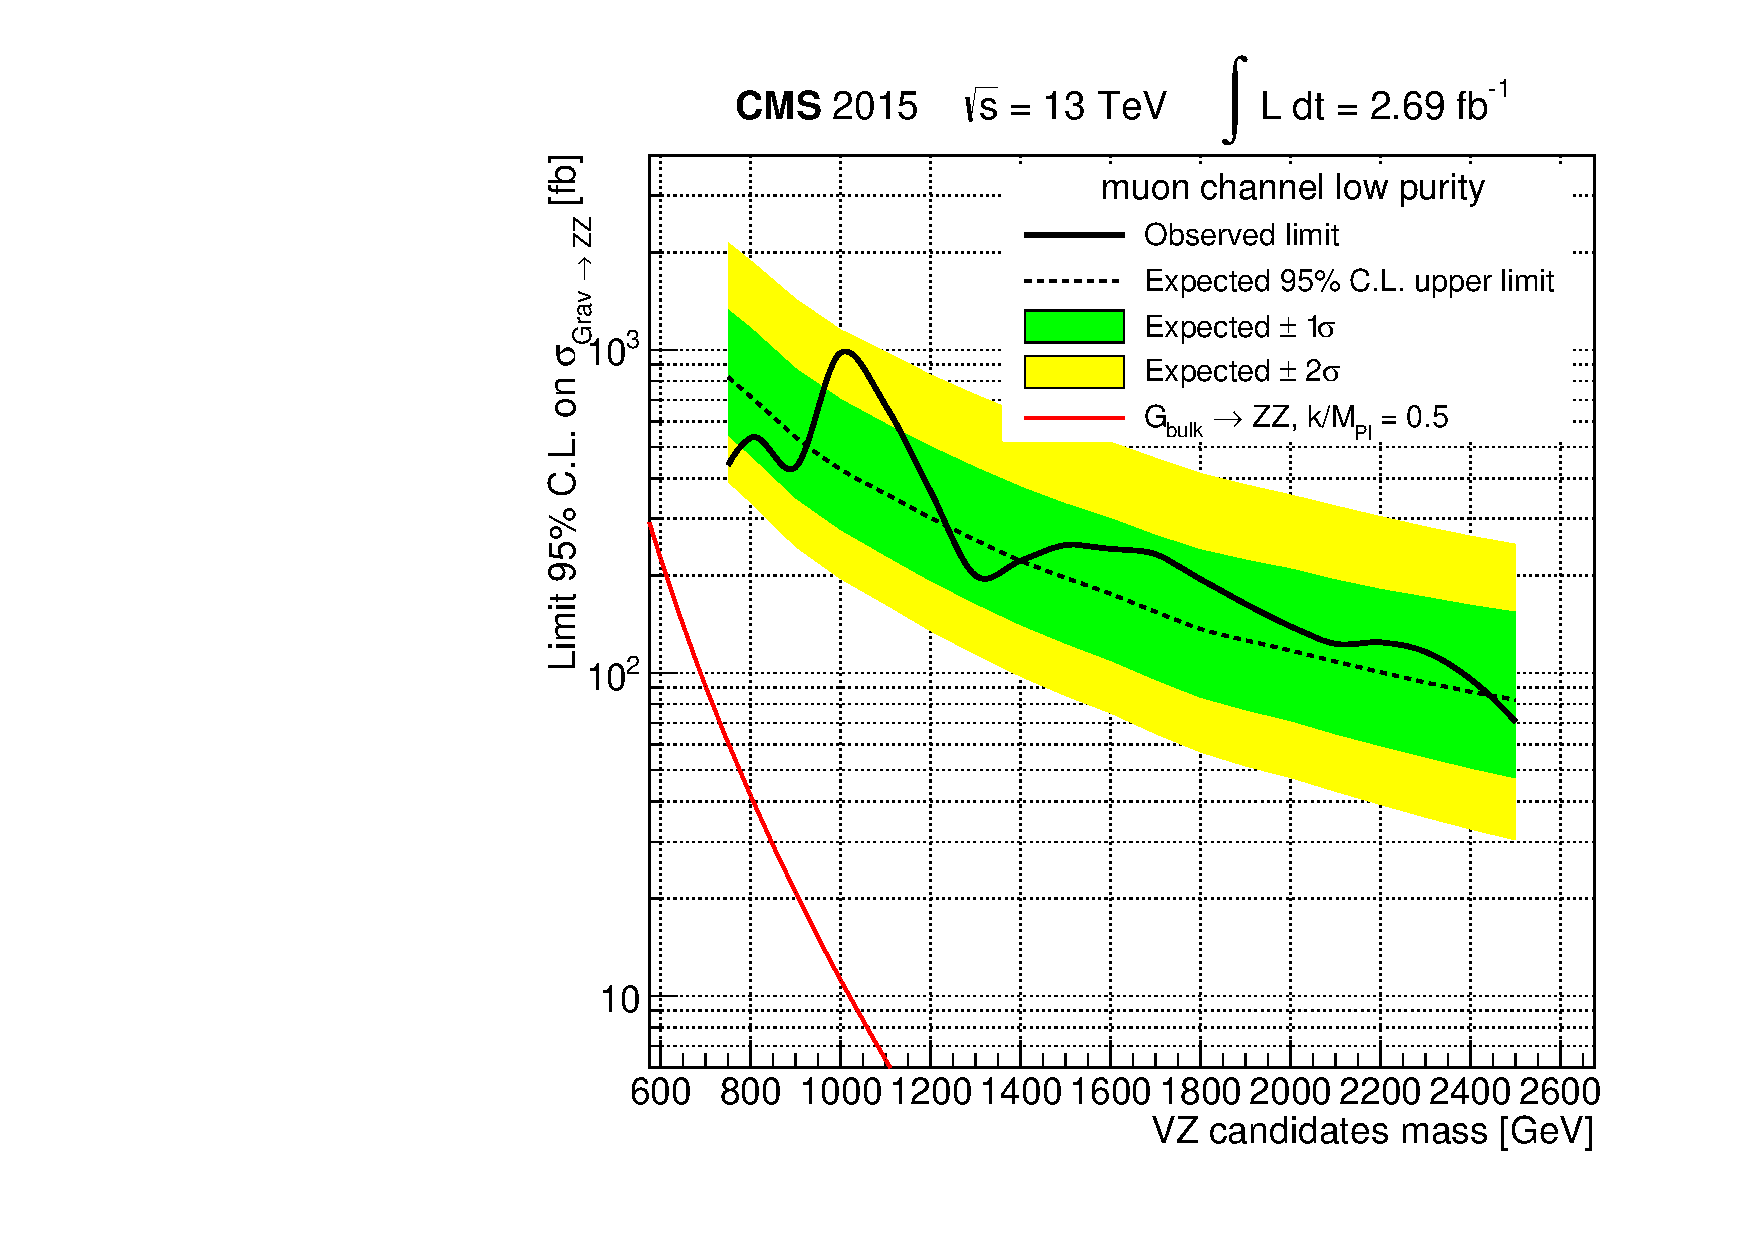
\includegraphics[scale=0.37]{figures/limits/limitMLP.pdf}
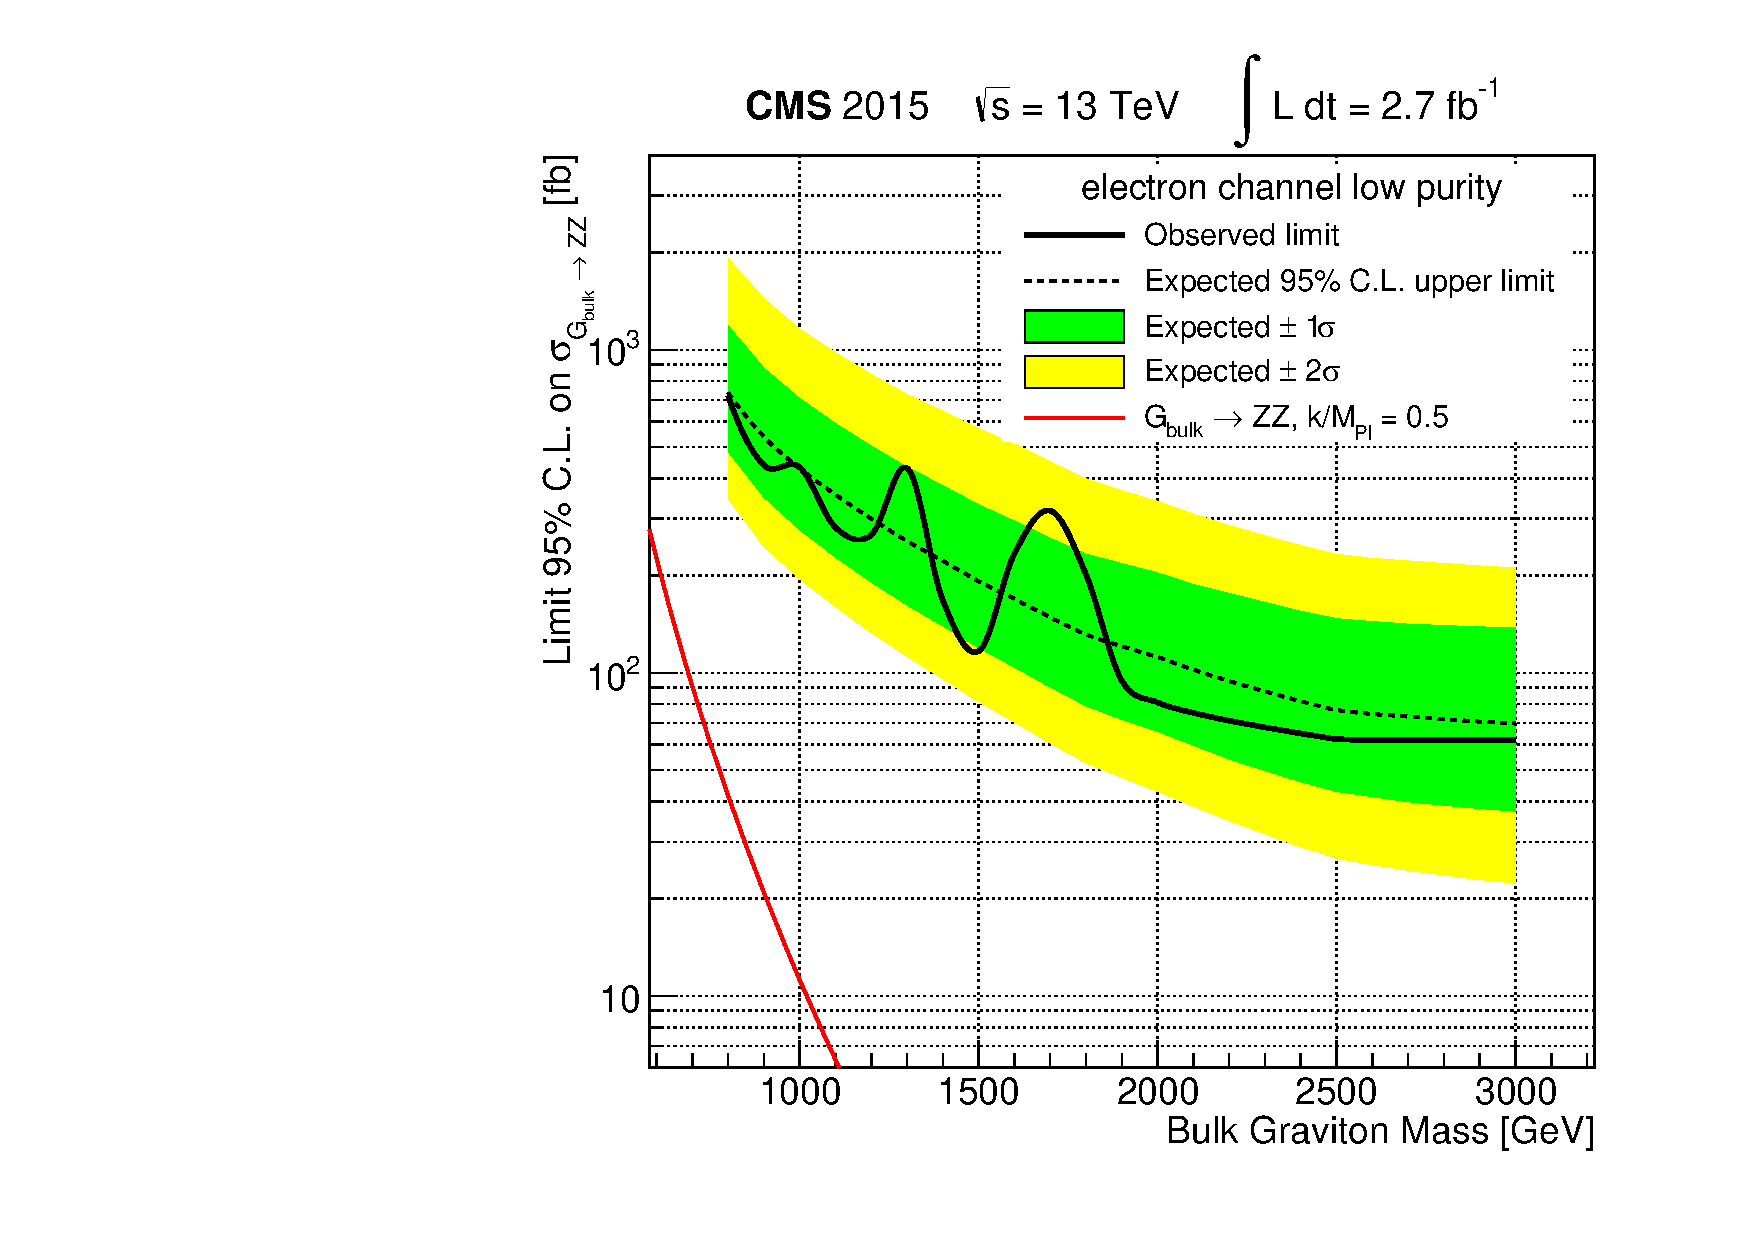
\includegraphics[scale=0.37]{figures/limits/limitELP.pdf}\\[1cm]
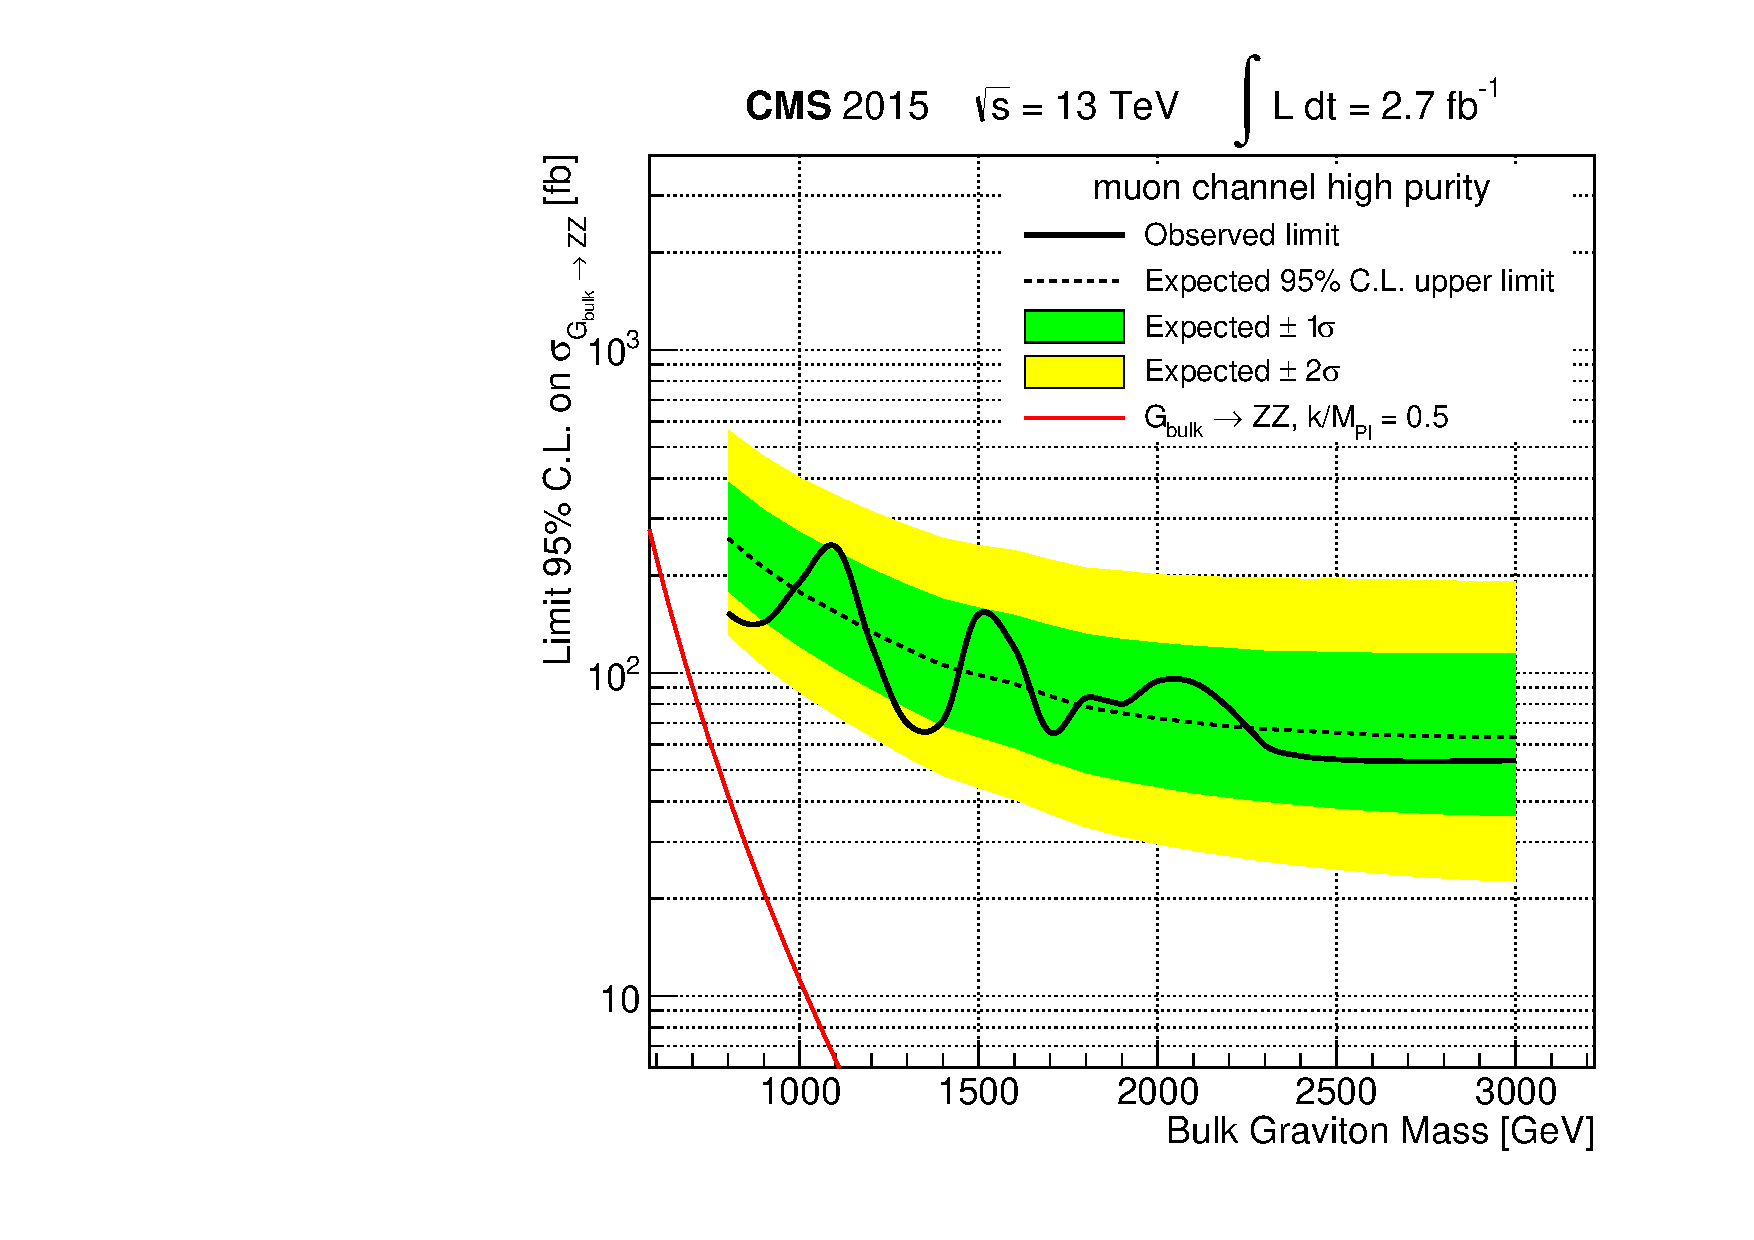
\includegraphics[scale=0.37]{figures/limits/limitMHP.pdf}
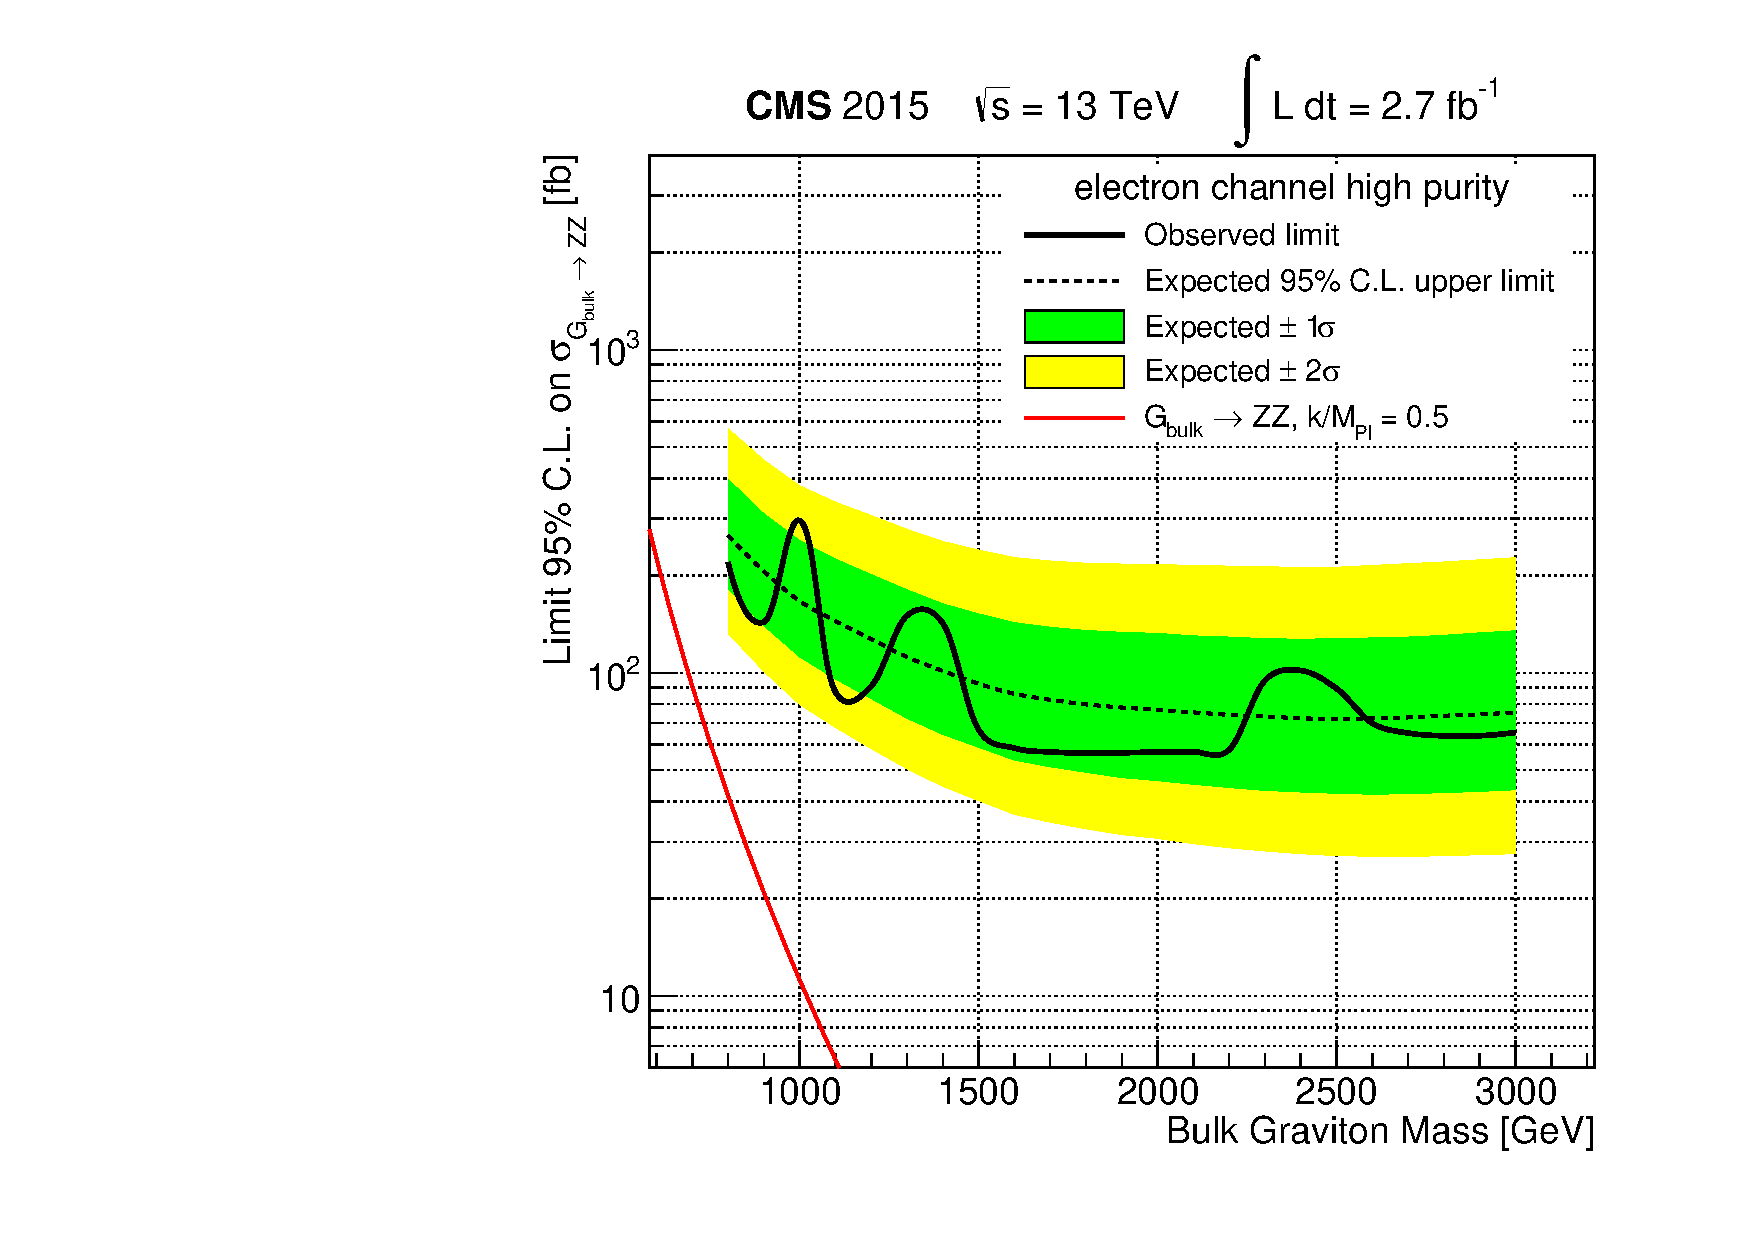
\includegraphics[scale=0.37]{figures/limits/limitEHP.pdf}
\caption[Upper limits per category]{Upper limits in the categories: muon low purity (top-left), electron low purity (top-right), muon high purity (bottom-left), and electron high purity (bottom-right.)}
\label{limits_VZ}
\end{figure}

Finally, the product of the likelihoods between the different categories is computed to combine the individual limits and obtain a more sensitive result, as shown in Fig. \ref{combine_VZ}.
\begin{figure}[h]
\centering
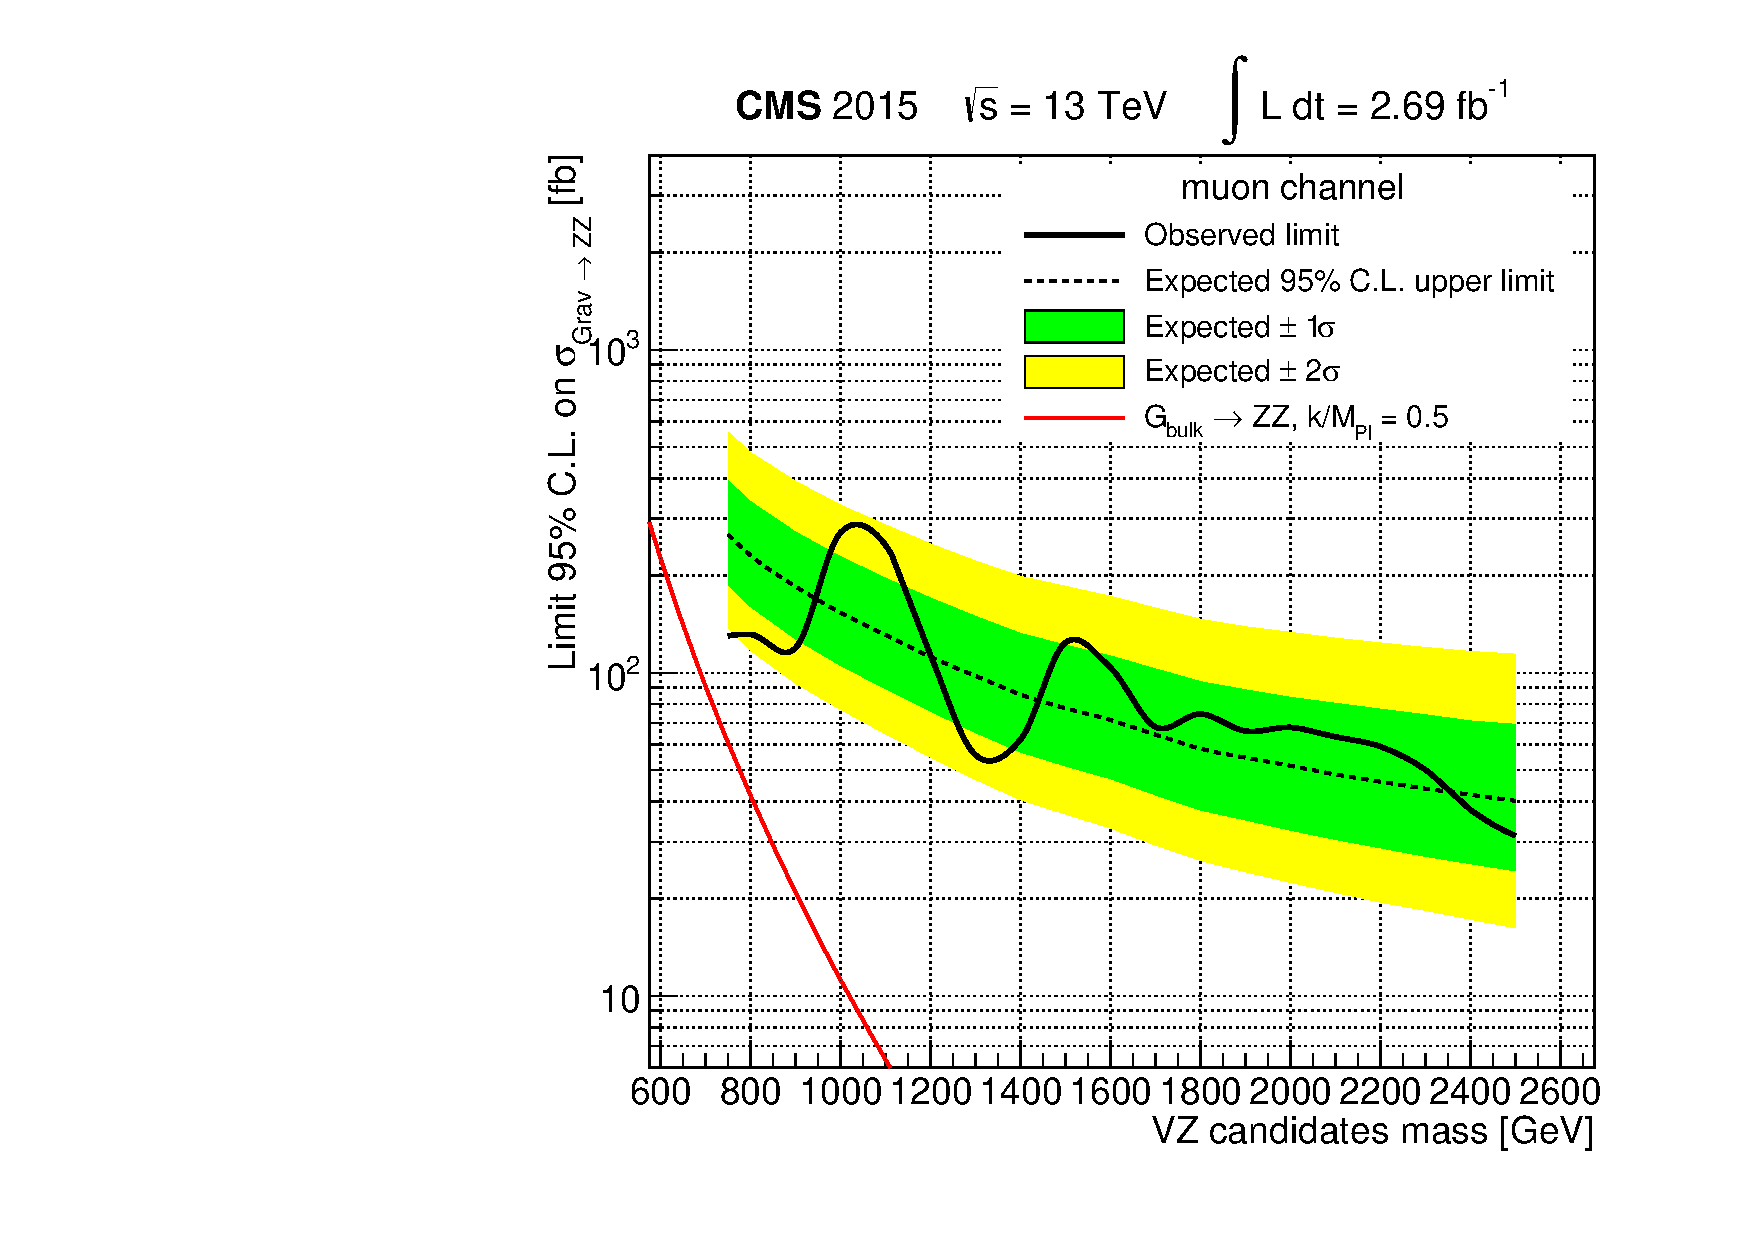
\includegraphics[scale=0.37]{figures/limits/limitMNP.pdf}
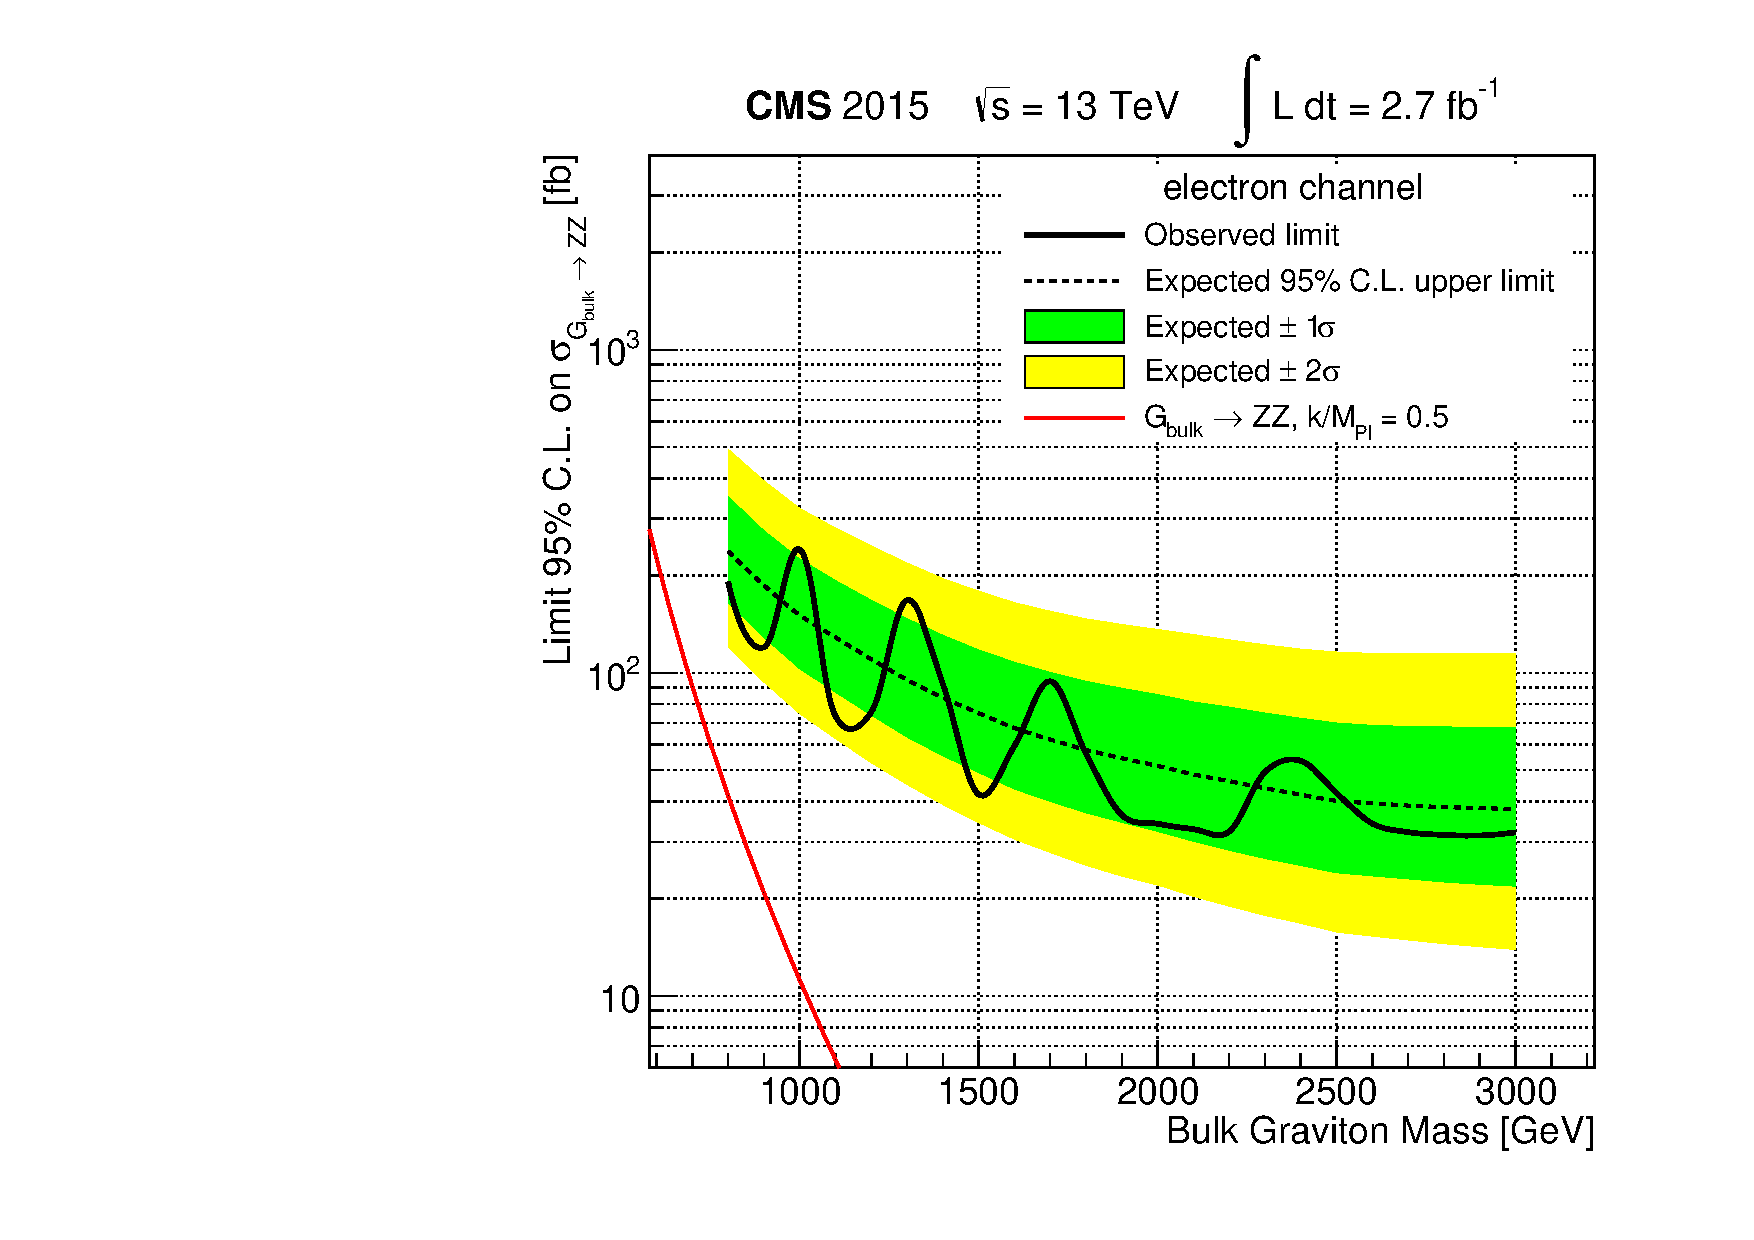
\includegraphics[scale=0.37]{figures/limits/limitENP.pdf}\\
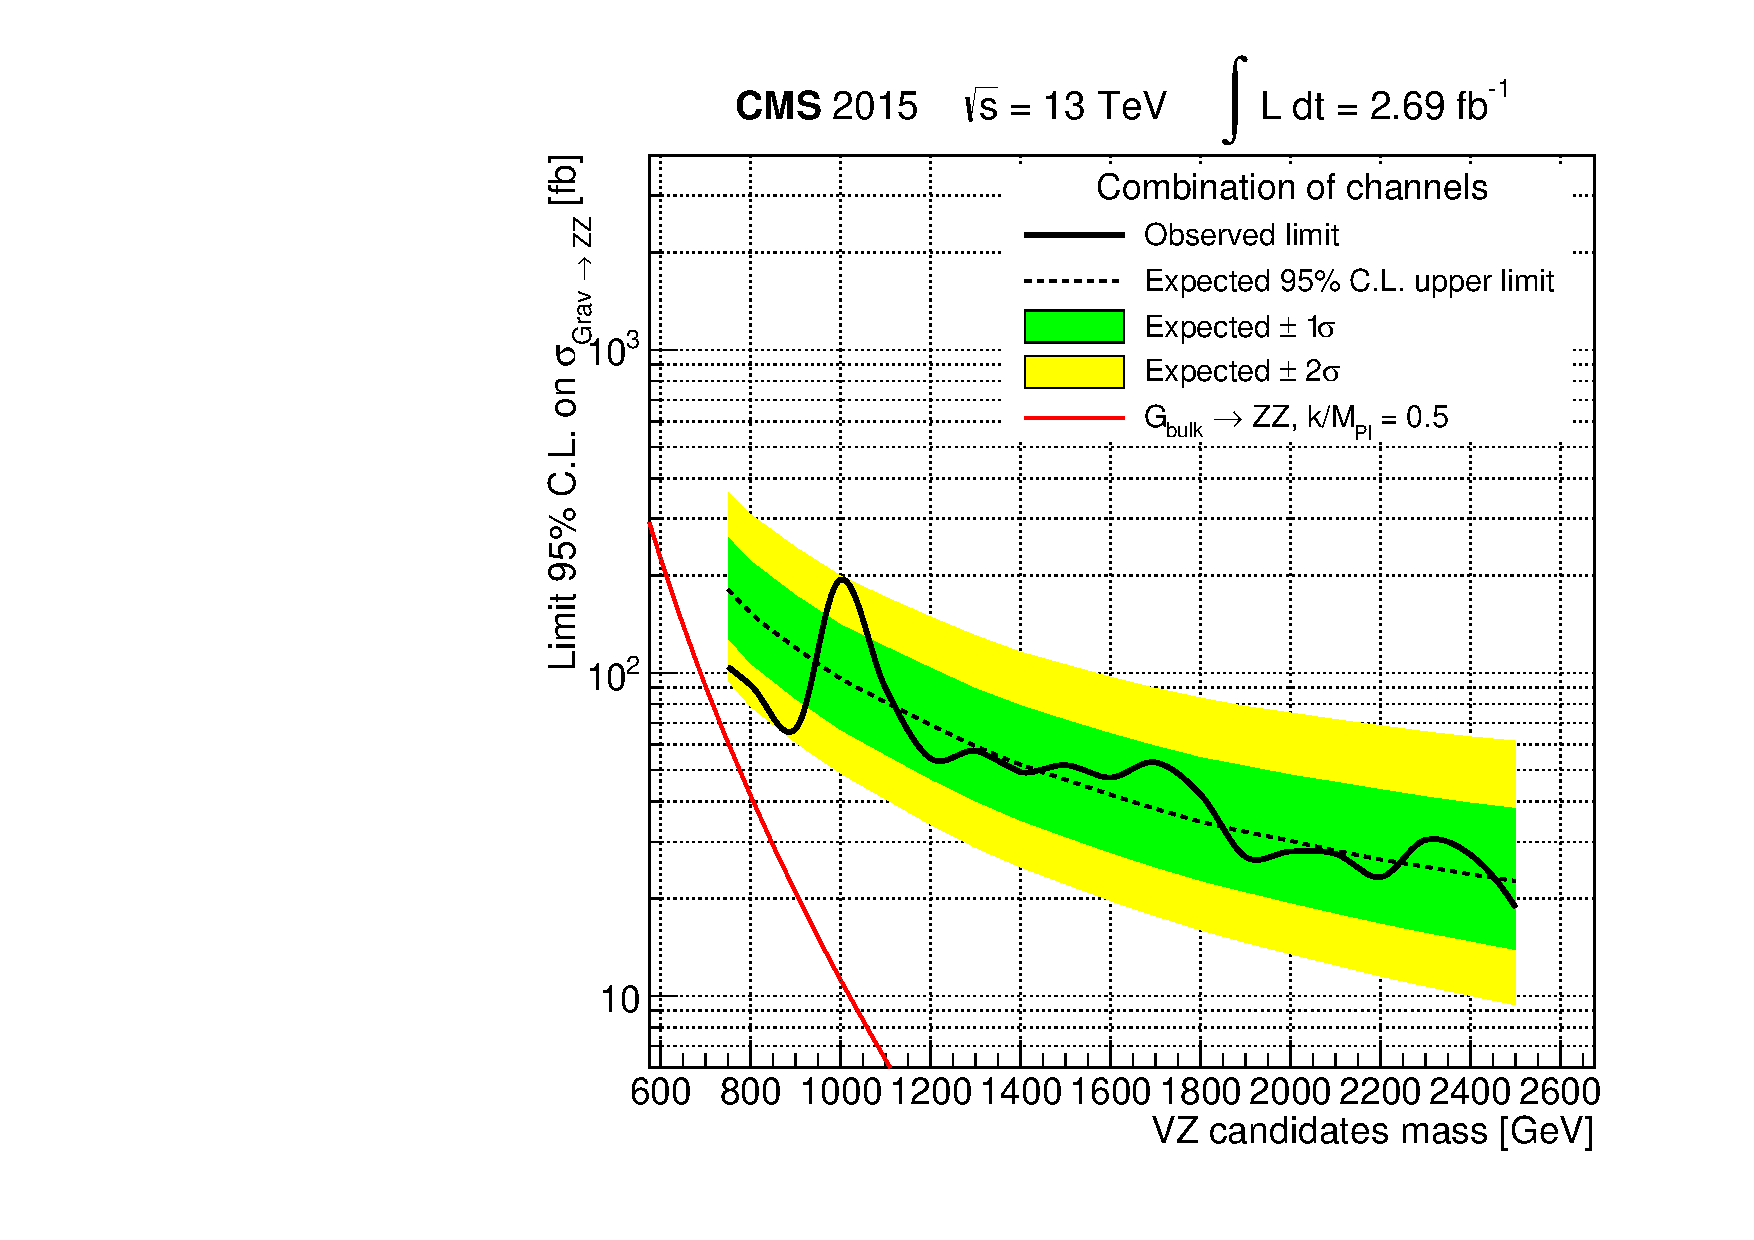
\includegraphics[scale=0.65]{figures/limits/limitANP.pdf}
\caption[Upper limits combination]{Upper limits obtained after combination of the high and low purity categories in the muon channel (top-left), electron electron channel (top-right), and the combination of all categories (bottom).}
\label{combine_VZ}
\end{figure}

\clearpage
\section{Interpretation of Results}
The final limit in Fig.~\ref{combine_VZ} combines all categories: muon low purity, electron low purity, muon high purity, and electron high purity. When the observed limit is above the expected value, it is possible to claim an excess over the standard model background. The significance of an excess is evaluated through the p-value, that is the incompatibility of the background-only hypothesis with the observed data. According to Fig.~\ref{significance}, the most significant point is found at 1 TeV corresponding to a p-value = 0.018. The p-value is often converted into a number of standard deviations of a gaussian distribution; if the significance is larger than $5\sigma$, an announcement of discovery can be made. Our particular excess in 1 TeV corresponds to a significance of $2\sigma$, as the solid line in Fig.~\ref{combine_VZ} just touches the upper yellow band.

\begin{figure}[h]
\centering
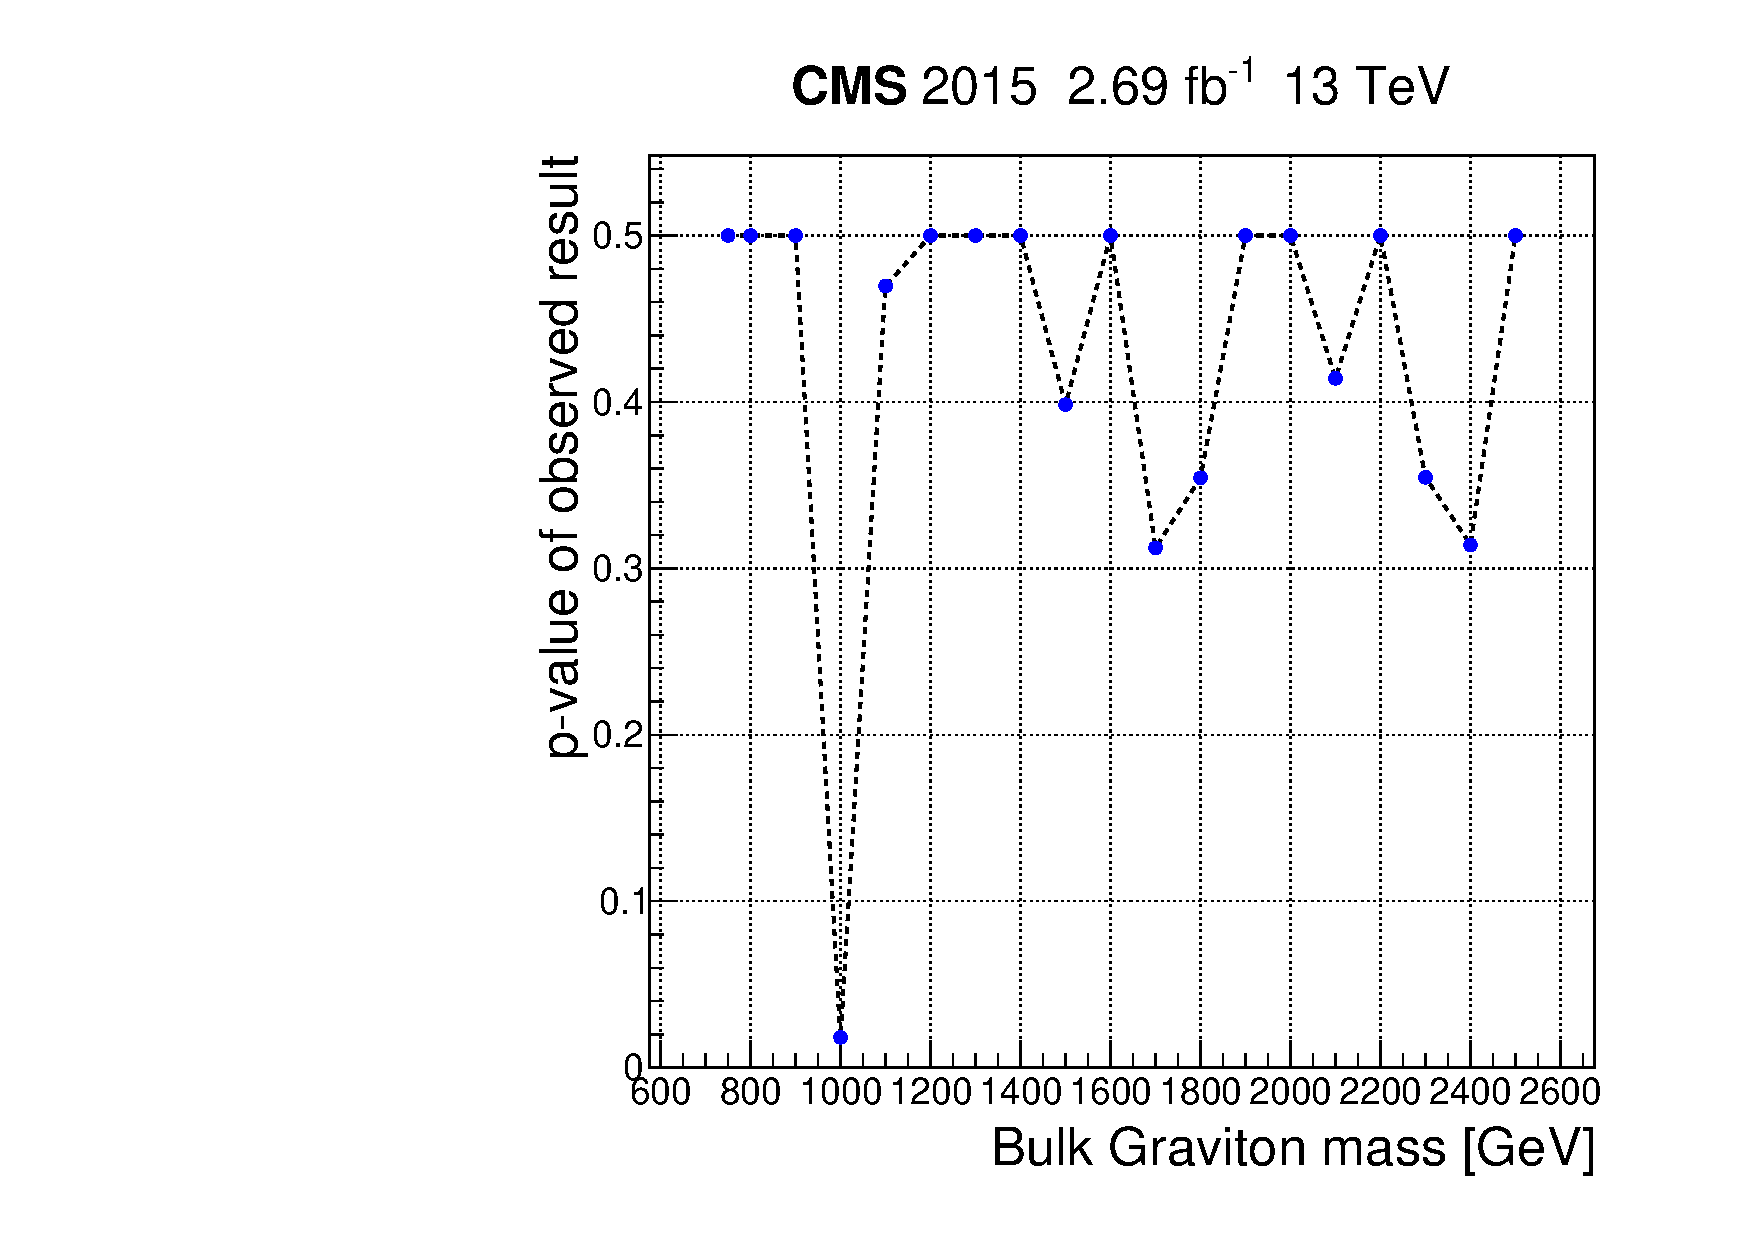
\includegraphics[scale=0.5]{figures/limits/signifANP.pdf}
\caption[Significance]{Significance of the observed results. The most significant result corresponds to the lowest p-value, observed at 1 TeV.}
\label{significance}
\end{figure}

The impacts of the nuisance parameters on the signal strength for the 1 TeV point are shown in Fig.~\ref{impacts}. The direction of the $+1$ sigma and $-1$ sigma impacts indicates whether the parameter is correlated or anti-correlated with the variation of the signal strength.

\begin{figure}[h]
\centering
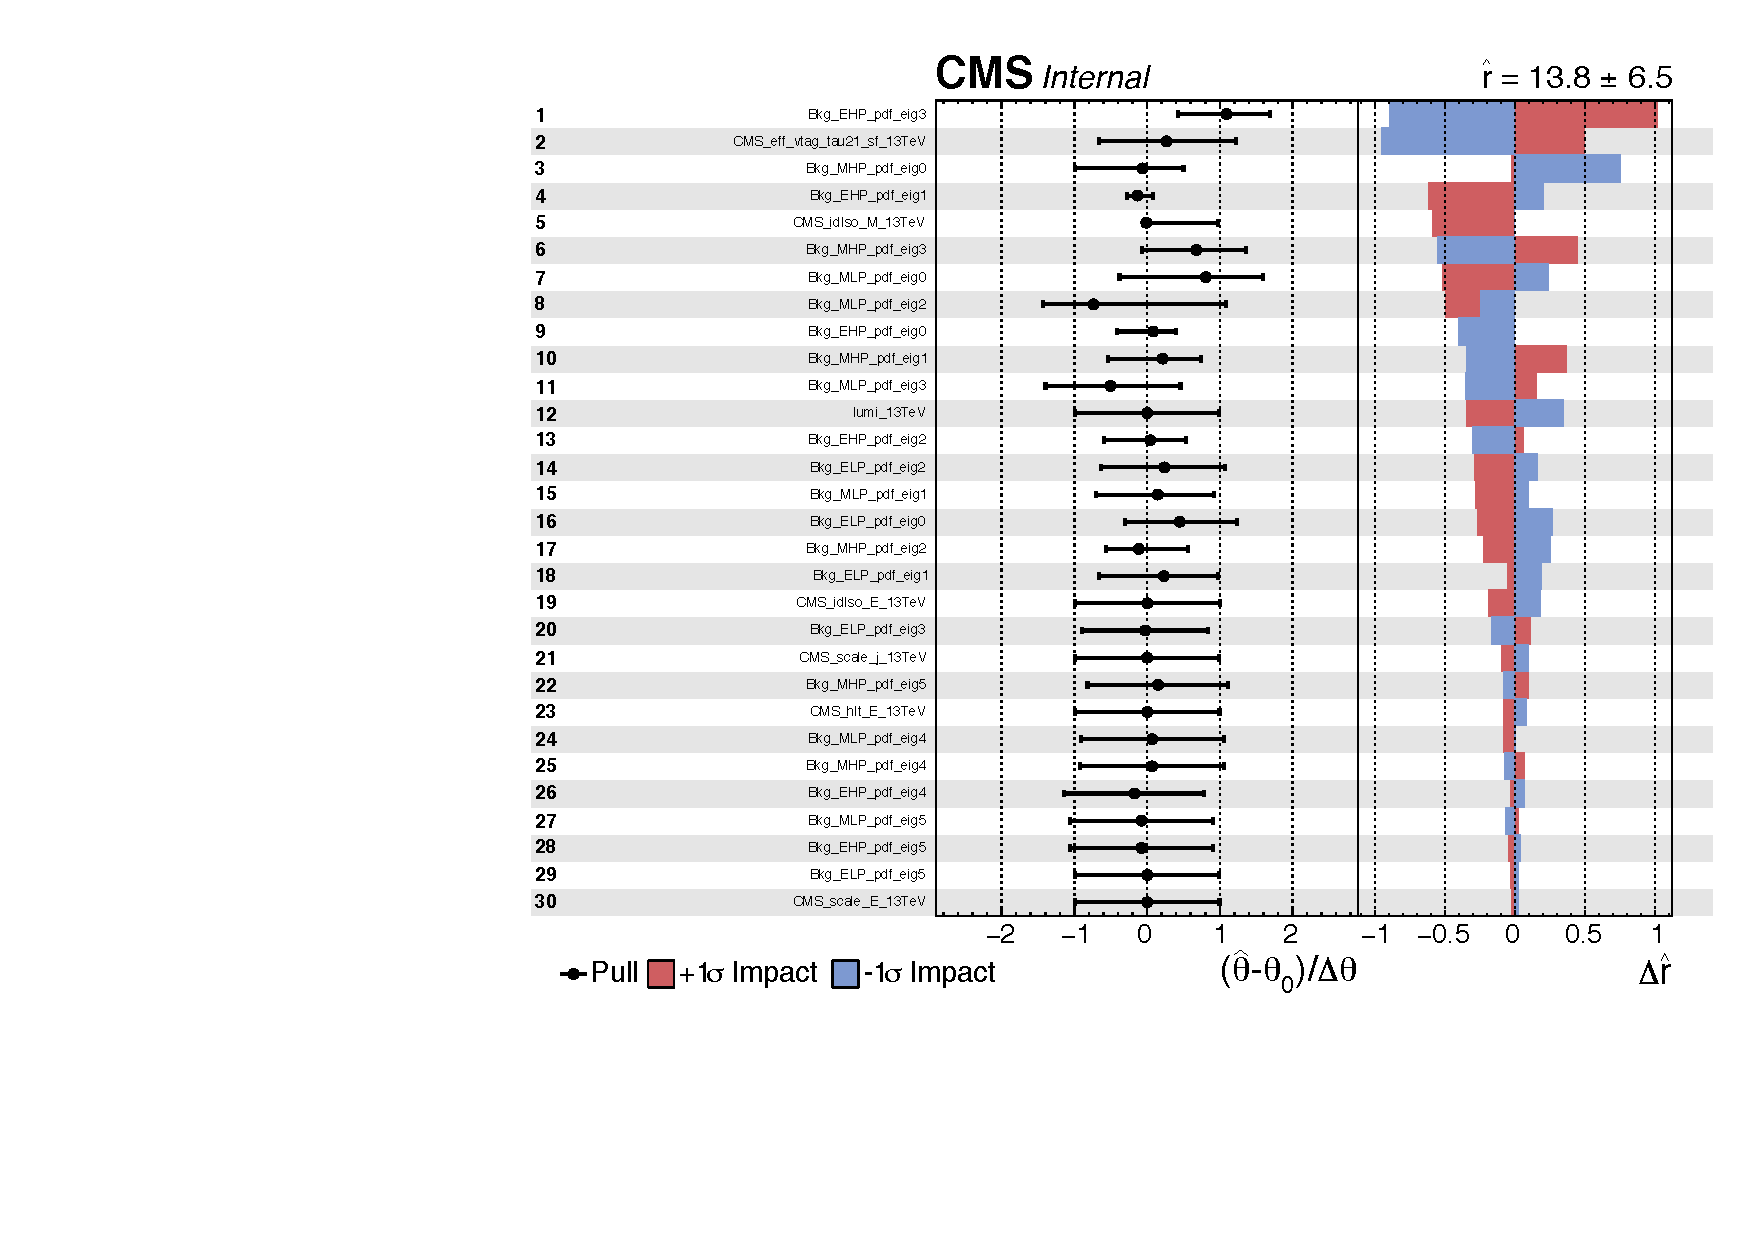
\includegraphics[scale=0.65]{figures/limits/impacts_1000_ANP_1.pdf}\\
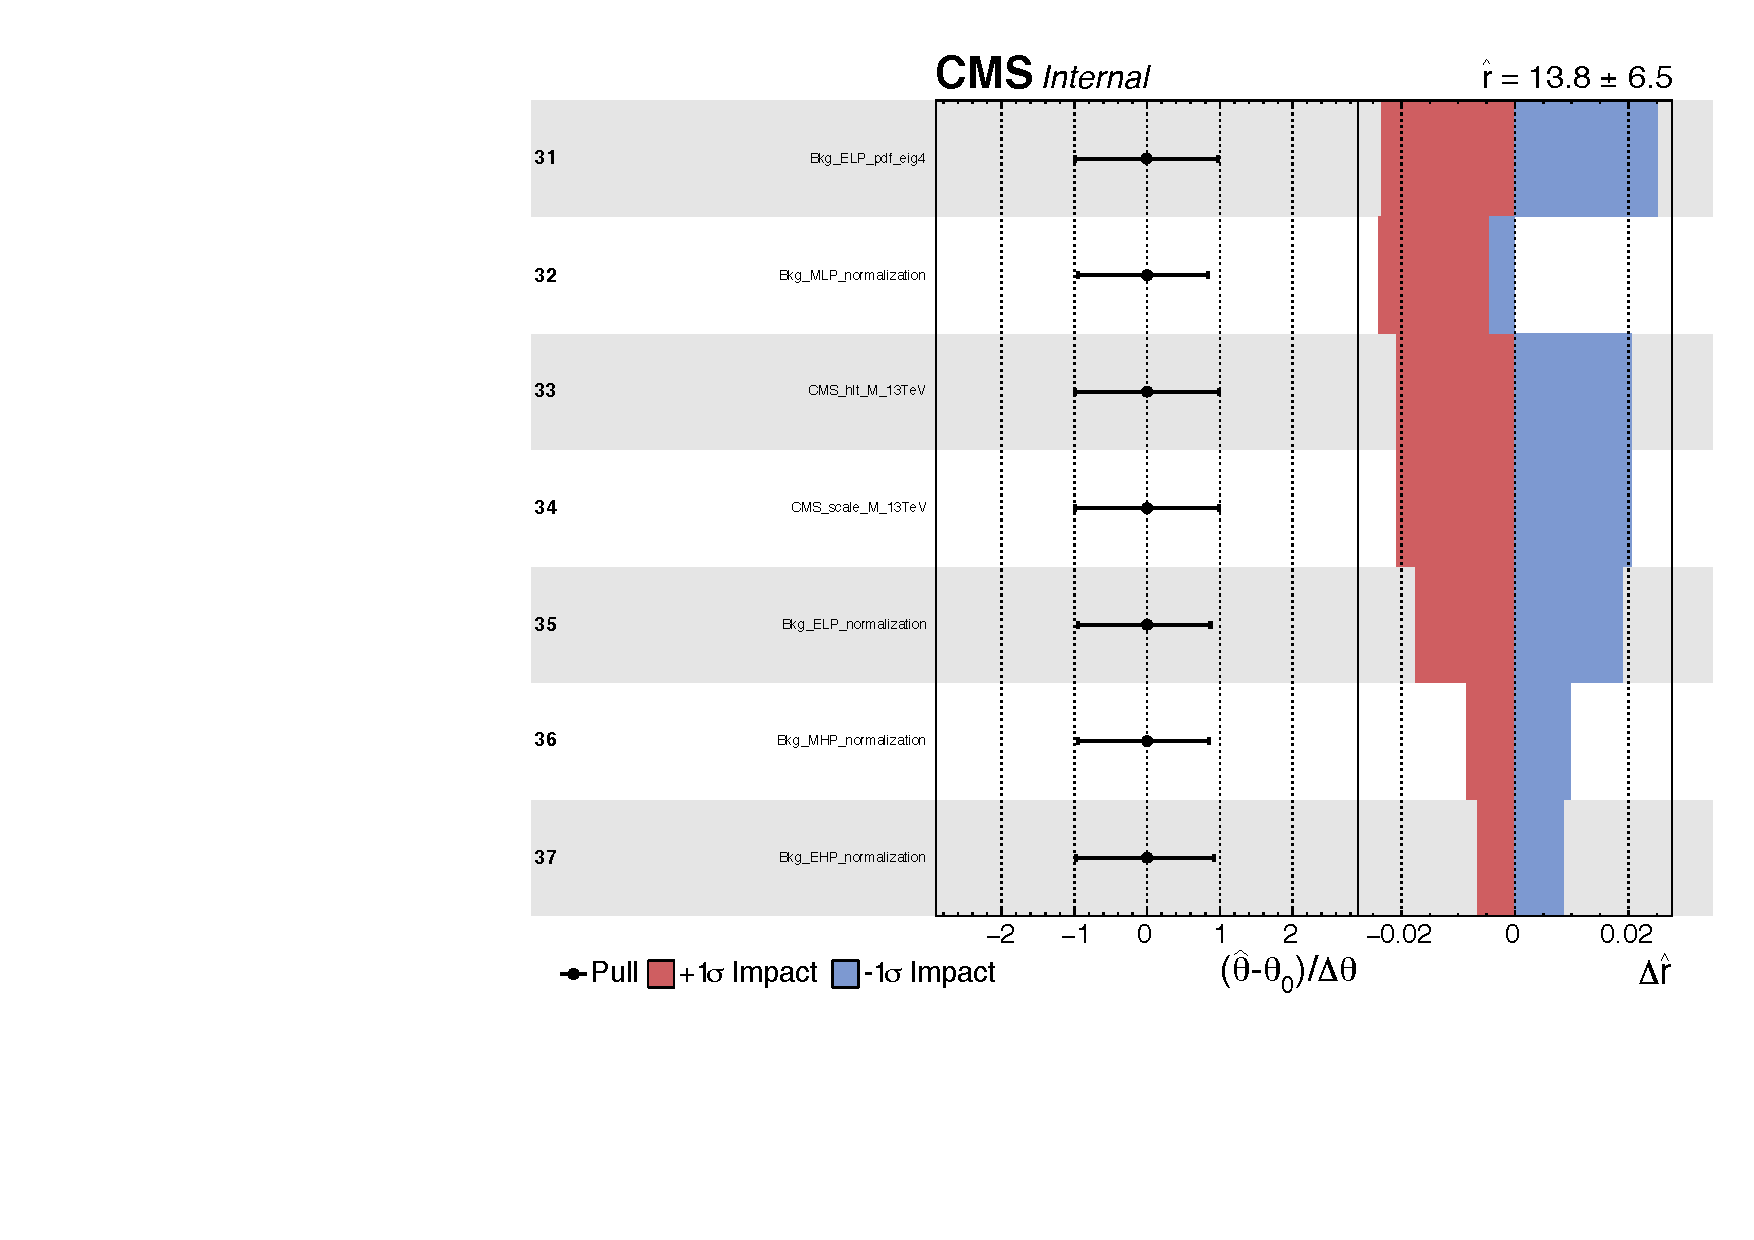
\includegraphics[scale=0.65]{figures/limits/impacts_1000_ANP_2.pdf}
\caption[Nuisance parameters]{Impacts on signal strength for point at 1 TeV.}
\label{impacts}
\end{figure}
